


\usetikzlibrary{calc}




\newcommand{\drawgrid}[5][]{%
\draw[line cap=rect,#1] (#2,#3) grid ++ (#4,#5); 
}

\newcommand{\drawrect}[5][]{%
\draw[line cap=rect,#1] (#2,#3) rectangle ++ (#4,#5); 
}


\newcommand{\fillcoord}[2]{%
\fill[black] (#1,#2) rectangle ++ (1,1); 
}

\newcommand{\namecoord}[4]{%
\node[label=center:#4] (#3) at ($(#1,#2)+(0.5,0.5)$) {}; 
}


\newcommand{\selectcoord}[2]{%
\draw[color=red, line width=1pt, line cap=rect]  (#1,#2) grid ($(#1,#2)+(1,1)$) {}; 
}

\newcommand{\linkcoord}[5][]{%
\draw[->,color=red, line width=1pt, line cap=rect,#1]  ($(#2,#3)+(0.5,0.5)$) -- ($(#4,#5)+(0.5,0.5)$) {}; 
}





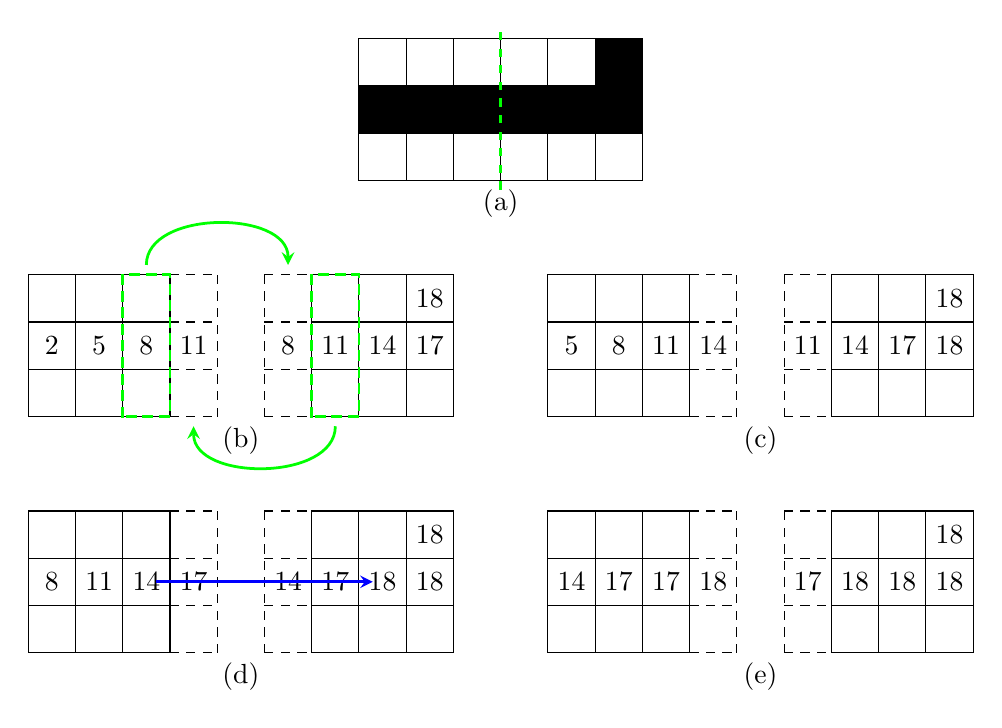
\begin{tikzpicture}[scale=0.6]


\begin{scope}[shift={(7,5)}]
\namecoord{2.5}{-1}{}{(a)}


\drawgrid{0}{0}{6}{3}

\fillcoord{0}{1}
\fillcoord{1}{1}
\fillcoord{2}{1}
\fillcoord{3}{1}
\fillcoord{4}{1}
\fillcoord{5}{1}
\fillcoord{5}{2}

\draw[dashed,green,line width=1pt] (3,-0.2) -- (3,3.2);
\end{scope}



\begin{scope}[shift={(0,0)}]
\namecoord{4}{-1}{}{(b)}


\drawgrid{0}{0}{3}{3}
\drawgrid{6}{0}{3}{3}

\drawgrid[dashed]{3}{0}{1}{3}
\drawrect[green,dashed, line width=1pt]{2}{0}{1}{3}
\drawgrid[dashed]{5}{0}{1}{3}
\drawrect[green,dashed, line width=1pt]{6}{0}{1}{3}

% \foreach \i in {0,...,8}
% \foreach \j in {0,...,2}
% {
% \namecoord{\i}{\j}{\i\j}{\i\j}
% }


\node[minimum size=0pt] (boundEast) at (5.5,3) {};
\node[minimum size=0pt] (boundWest) at (2.5,3) {};
\draw[-stealth,color=green, line width=1pt] (boundWest) edge [in=90, out=90] (boundEast);

\node[minimum size=0pt] (boundEast) at (6.5,0) {};
\node[minimum size=0pt] (boundWest) at (3.5,0) {};
\draw[-stealth,color=green, line width=1pt] (boundEast) edge [in=-90, out=-90] (boundWest);


\namecoord{0}{1}{}{2}
\namecoord{1}{1}{}{5}
\namecoord{2}{1}{}{8}
\namecoord{3}{1}{}{11}

\namecoord{5}{1}{}{8}
\namecoord{6}{1}{}{11}
\namecoord{7}{1}{}{14}
\namecoord{8}{1}{}{17}
\namecoord{8}{2}{}{18}

\end{scope}


\begin{scope}[shift={(11,0)}]
\namecoord{4}{-1}{}{(c)}


\drawgrid{0}{0}{3}{3}
\drawgrid{6}{0}{3}{3}

\drawgrid[dashed]{3}{0}{1}{3}
% \drawrect[green,dashed, line width=1pt]{2}{0}{1}{3}
\drawgrid[dashed]{5}{0}{1}{3}
% \drawrect[green,dashed, line width=1pt]{6}{0}{1}{3}



\namecoord{0}{1}{}{5}
\namecoord{1}{1}{}{8}
\namecoord{2}{1}{}{11}
\namecoord{3}{1}{}{14}

\namecoord{5}{1}{}{11}
\namecoord{6}{1}{}{14}
\namecoord{7}{1}{}{17}
\namecoord{8}{1}{}{18}
\namecoord{8}{2}{}{18}

\end{scope}

\begin{scope}[shift={(0,-5)}]
\namecoord{4}{-1}{}{(d)}


\drawgrid{0}{0}{3}{3}
\drawgrid{6}{0}{3}{3}

\drawgrid[dashed]{3}{0}{1}{3}
% \drawrect[green,dashed, line width=1pt]{2}{0}{1}{3}
\drawgrid[dashed]{5}{0}{1}{3}
% \drawrect[green,dashed, line width=1pt]{6}{0}{1}{3}



\namecoord{0}{1}{}{8}
\namecoord{1}{1}{}{11}
\namecoord{2}{1}{21}{14}
\namecoord{3}{1}{}{17}

\namecoord{5}{1}{51}{14}
\namecoord{6}{1}{}{17}
\namecoord{7}{1}{71}{18}
\namecoord{8}{1}{}{18}
\namecoord{8}{2}{}{18}

\draw[-stealth,color=blue, line width=1pt] (21) -- (71);
\end{scope}

\begin{scope}[shift={(11,-5)}]
\namecoord{4}{-1}{}{(e)}


\drawgrid{0}{0}{3}{3}
\drawgrid{6}{0}{3}{3}

\drawgrid[dashed]{3}{0}{1}{3}
% \drawrect[green,dashed, line width=1pt]{2}{0}{1}{3}
\drawgrid[dashed]{5}{0}{1}{3}
% \drawrect[green,dashed, line width=1pt]{6}{0}{1}{3}



\namecoord{0}{1}{}{14}
\namecoord{1}{1}{}{17}
\namecoord{2}{1}{21}{17}
\namecoord{3}{1}{}{18}

\namecoord{5}{1}{51}{17}
\namecoord{6}{1}{}{18}
\namecoord{7}{1}{71}{18}
\namecoord{8}{1}{}{18}
\namecoord{8}{2}{}{18}

% \draw[-stealth,color=blue, line width=1pt] (21) -- (71);
\end{scope}

\end{tikzpicture}



